\subsection{Wikidata}

Wikidata is the free and open knowledge base by the Wikimedia movement, which collects multilingual structured data in one central place and makes it publicly available under CC0, a public domain dedication. \footnote{\href{https://creativecommons.org/publicdomain/zero/1.0/}{https://creativecommons.org/publicdomain/zero/1.0/}} Similar to the Wikipedia it can be edited by anyone. Wikidata collects data on different topics like people, places, events and many more.
\begin{figure}[ht]
	\centering
	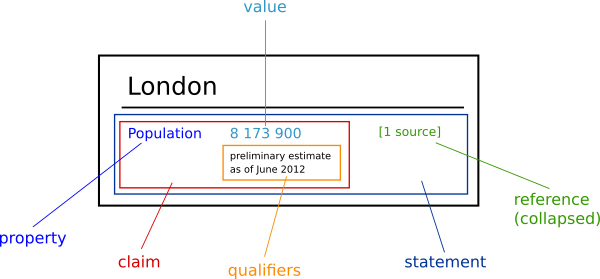
\includegraphics[width=120mm]{diagrams/Wikidata_statement.png}
	\caption{Wikidata Statement for item London}
	\label{fig1}
\end{figure}

Every item has a unique identifier, starting with the letter ``Q'' followed by a number unique to the item. Therefore it is clearly identifiable and not depending on labels, which may change. \\
Statements contain a property, which is the core part and indicating, what kind of statement is made. One or more values are attached to this property. For example, a statement for a city could be the property ``Population'' (P123) \todo{correct property id} with the according number of inhabitants. There can be multiple values for population of different years, differentiated by qualifiers. To identify the important and most recent data, the values can be marked as preferred, normal and deprecated.\\
Data types for the properties \todo{explain properties before as well as triples!} are items, string, quantity, names of Wikimedia Commons files, geo coordinate, time, URL,  and in the future also identifier of other databases like VIAF. \\
The data is published under CC-0 and therefore free to anyone to copy, use and distribute.
The aim is not only to have a knowledge base that supports Wikipedia but can also be used in other contexts in the semantic web. Therefore, Wikidata offers an API as well as a SPARQL endpoint. Additionally, the data can be downloaded as a full database dump in the formats JSON, XML and RDF.  